\documentclass[a4paper]{article}

\usepackage[hidelinks]{hyperref} % Clickable links in PDF.
\usepackage[margin=2.8cm]{geometry}
\usepackage{graphicx}

\begin{document}
\pagestyle{empty}


Working and training different network architectures made me understand that neural networks are not easily applied to every problem. Changing the hyperparameters slightly might result in a network that will not train at all, like the blur kernel size. Also much care needs to be taken when defining the loss function. Applying the color rebalancing resulted higher saturated images, giving more perceptual realistic images. Having a probabilistic outcome for each pixel gives more freedom in the post-processing. Now annealed mean is applied, which gives very good results, solving the averaging problem. However, the network is not always aware of each object and uses two distinct colors to color the same object i.e. a pepper that can be green or orange is colored both on different locations as in figure \ref{fig:color}. Image segmentation could be used by applying the annealed mean over the joint probability of each segment.\\

\begin{figure}[h]
	\centering
	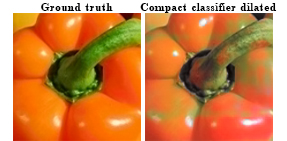
\includegraphics[width=0.35\textwidth]{plaatje}
	\caption{The problem of having the right color, but not uniform over the same object.}
	\label{fig:color}
\end{figure}

A specific problem for segmentation like convolutional neural networks, is the maintainability of spacial information. Two different methods are used, convolution with strides and concatenation of local and global features. Even though differences in the results are marginal, the network that uses strides shows less artifacts. An explanation could be that it is easier to determine the position of certain features if the scaled position remains the same, as is by applying strides. With concatenation the extracted features need to be rematched to the input. Interestingly the combination of strides and concatenation shows even less artifacts, however the dataset seems to be too limited to give proper results. Therefore it is recommended to train an architecture like that on a bigger dataset.  \\

Once all the left over details are solved for the colorization network, and it can successfully color almost any object (training on ImageNet or just a lot of random images from the internet), then there are two interesting applications. The first being a combination with one of the colorization algorithms that need user input. Those algorithms work very well on high resolution images. By using an upscaled neural network output as the input for one of those algorithms, the whole system will become a high resolution colorization network. It would of course be possible to pass a higher resolution image through the network as is, but it would likely result in more artifacts, unless the network is trained on higher resolution images, which will require a lot more computational power.

The second application would be to combine the network with a recurrent neural network, giving it the possibility to remember what it colored the last frame. That way the network can be used to colorize videos without the colorization of the same object, in different colors, in each successive frame\footnote{The algorithm from the paper Iizuka et al. is applied to various videos, clearly showing different colors every frame, one of which can be found on YouTube: \url{https://youtu.be/GNUeri_PQdk?list=PLoHIT_YpaTX-hGOpaM0-zHEtwX8DnWM5x}}. Combining this with the first application would provide a fully automatic system to colorize high resolution video.\\

Starting this project there was only one publication of using a neural network to colorize images. Now at the end, there are a handful of papers published, all in 2016. Certain methods and layers used in our architectures are also very recent additions, like the batch normalization and the dilated convolution. This just shows that the machine learning community is very fast paced with nearly endless possibilities. Personally I think many future products will use some form of machine learning and I would like to have my share in it. \\

Dawud Hage

4190696



 \end{document}


